\documentclass[border=10pt]{standalone}

% colour definitions
\usepackage{xcolor}
\definecolor{myblue}{rgb}{0, 0, 0.8}
\definecolor{darkgreen}{rgb}{0, 0.8, 0}

% for diagrams
\usepackage{tikz}
\usetikzlibrary{shadings, intersections, positioning, arrows}
\usetikzlibrary{decorations.pathmorphing}
\usetikzlibrary{decorations.markings}
\usetikzlibrary{decorations.pathreplacing}
\usetikzlibrary{shapes.misc}
\usetikzlibrary{shadows.blur}

%\usetikzlibrary{external}
%\tikzexternalize[prefix=build/]

% common things used for feynman diagrams
% NOTE, these are defined here, but when the figuresare used from within my thesis directory, the definitions there will be used!!

\tikzset{
	particle/.style={thick,draw=black, postaction={decorate},
	decoration={markings,mark=at position .5 with {\arrow[black]{triangle 45}}}}
}


\newcommand{\tauHad}{\ensuremath{\tau_\mathrm{had}}}
\newcommand{\tauhad}{\tauHad}
\newcommand{\MET}{\ensuremath{E_\mathrm{T}^\mathrm{miss.}}}

\tikzset{
	particleNoArrow/.style={thick,draw=black, postaction={decorate}}
}

\tikzset{
	Wboson/.style={decorate, draw=black,
	decoration={coil,aspect=0}}
}

\tikzset{
	gluon/.style={decorate, draw=black,
    decoration={coil,aspect=0.3,segment length=3pt,amplitude=3pt}}
 }

\begin{document}
	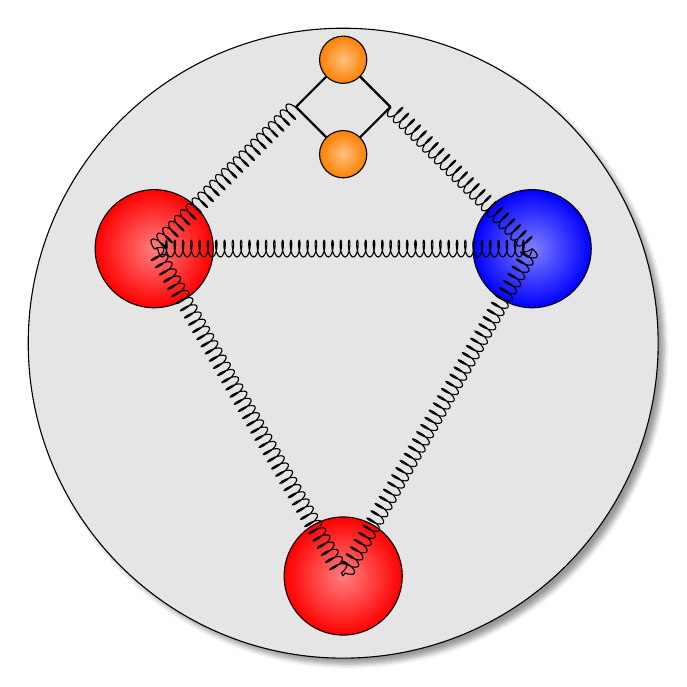
\begin{tikzpicture}[x=1.2cm, y=1.2cm]
		
		% origin for main proton circle
		\newcommand{\xreference}{0}
		\newcommand{\yreference}{0}
		\newcommand{\protonradius}{4cm}
		\newcommand{\quarkradius}{5cm * 0.15}
		\newcommand{\seaquarkradius}{\quarkradius * 0.4}
		\newcommand{\offset}{2}

		% proton
		\filldraw[blur shadow={shadow blur steps=5}, color=gray!20, draw=black] (\xreference, \yreference + 1) circle (\protonradius);

		% valence quarks
		\shadedraw[inner color=blue!50, outer color=blue, draw=black] (\xreference + \offset, \yreference + \offset) circle (\quarkradius);
		\shadedraw[inner color=red!50, outer color=red, draw=black] (\xreference - \offset, \yreference + \offset) circle (\quarkradius);
		% from Pythagorous: down offset is sqrt(3) * x offset - y offset = (sqrt(3) - 1) * offset
		\newcommand{\ylowerquark}{0.73205080757 * \offset}
		\shadedraw[inner color=red!50, outer color=red, draw=black] (\xreference, -1 * \ylowerquark) circle (\quarkradius);

		%% labels
		%\newcommand{\labeloffset}{0.25}
		%\node at (\xreference + \offset + \labeloffset, \yreference + \offset + \labeloffset) {\color{white}\Large{u}};
		%\node at (\xreference - \offset - \labeloffset, \yreference + \offset + \labeloffset) {\color{white}\Large{d}};
		%% from Pythagorous: sqrt{3}x - y
		%\node at (\xreference + 0, 3 * \xreference - \yreference) {\color{white}\Large{d}};
		
		\draw[gluon] (\xreference + \offset, \yreference + \offset) -- (\xreference - \offset, \yreference + \offset);
		\draw[gluon] (\xreference + \offset, \yreference + \offset) -- (\xreference, -1 * \ylowerquark);
		\draw[gluon] (\xreference - \offset, \yreference + \offset) -- (\xreference, -1 * \ylowerquark);

		% sea quarks
		% gluons
		\newcommand{\gluonoffset}{1.5}
		\draw[gluon] (\xreference + \offset, \yreference + \offset) -- (\xreference + \offset - \gluonoffset, \yreference + \offset + \gluonoffset);
		\draw[gluon] (\xreference - \offset, \yreference + \offset) -- (\xreference - \offset + \gluonoffset, \yreference + \offset + \gluonoffset);

		\draw[particleNoArrow] (\xreference + \offset - \gluonoffset, \yreference + \offset + \gluonoffset) -- (\xreference + \offset - \gluonoffset - 0.5, \yreference + \offset + \gluonoffset + 0.5);
		\draw[particleNoArrow] (\xreference + \offset - \gluonoffset, \yreference + \offset + \gluonoffset) -- (\xreference + \offset - \gluonoffset - 0.5, \yreference + \offset + \gluonoffset - 0.5);

		\draw[particleNoArrow] (\xreference - \offset + \gluonoffset, \yreference + \offset + \gluonoffset) -- (\xreference - \offset + \gluonoffset + 0.5, \yreference + \offset + \gluonoffset + 0.5);
		\draw[particleNoArrow] (\xreference - \offset + \gluonoffset, \yreference + \offset + \gluonoffset) -- (\xreference - \offset + \gluonoffset + 0.5, \yreference + \offset + \gluonoffset - 0.5);

		% quarks
		\shadedraw[inner color=orange!50, outer color=orange, draw=black] (\xreference, \yreference + 2 * \offset) circle (\seaquarkradius);
		\shadedraw[inner color=orange!50, outer color=orange, draw=black] (\xreference, \yreference + 1.5 * \offset) circle (\seaquarkradius);

	\end{tikzpicture}
\end{document}
